\documentclass[msc,numbers]{coppe}
\usepackage[utf8]{inputenc}
\usepackage{amsmath,amssymb}
\usepackage{hyperref}
\usepackage{pdflscape}

\makelosymbols
\makeloabbreviations

\begin{document}
  \title{Avaliação da dinâmica de um manipulador robótico sobre bases flexíveis}
  \foreigntitle{Thesis Title}
  \author{Estevão}{Fróes Ferrão}
  \advisor{Prof.}{Fernando}{ Augusto de Noronha Castro Pinto}{D.Sc.}
  %\advisor{Prof.}{Nome do Segundo Orientador}{Sobrenome}{Ph.D.}
  %\advisor{Prof.}{Nome do Terceiro Orientador}{Sobrenome}{D.Sc.}

  \examiner{Prof.}{Nome do Primeiro Examinador Sobrenome}{D.Sc.}
  \examiner{Prof.}{Nome do Segundo Examinador Sobrenome}{Ph.D.}
  \examiner{Prof.}{Nome do Terceiro Examinador Sobrenome}{D.Sc.}
  \examiner{Prof.}{Nome do Quarto Examinador Sobrenome}{Ph.D.}
  \examiner{Prof.}{Nome do Quinto Examinador Sobrenome}{Ph.D.}
  \department{PEM}
  \date{02}{2017}

  \keyword{Primeira palavra-chave}
  \keyword{Segunda palavra-chave}
  \keyword{Terceira palavra-chave}

  \maketitle
  
  %\frontmatter
  %\dedication{A algu\'em cujo valor \'e digno desta dedicat\'oria.}


  %\chapter*{Agradecimentos}

Gostaria de agradecer a todos.

  %\begin{abstract}

Apresenta-se, nesta tese, ...

\end{abstract}


  %\begin{foreignabstract}

In this work, we present ...

\end{foreignabstract}


  \tableofcontents
  %\listoffigures
  %\listoftables
  \printlosymbols
  \printloabbreviations

  \mainmatter
  \chapter{Introdução}

A aplicação da tecnologia de manipuladores robóticos se dá principalmente
em ambientes de automação industrial. Porém, cada vez mais robôs estão
substituindo humanos em serviços fora de um ambiente industrial e
estruturado\footnote{Ambiente estruturado: é o ambiente onde os parâmetros
necessários à operacionalidade do sistema robótico podem ser identificados e
quantificados.}. Quando a aplicação se dá em um ambiente de automação
industrial, este é chamado de robô industrial e quando se dá fora, ou
\textit{in situ}, este é chamado robô de serviço \cite{ISO8373}.

Apesar da grande variedade disponível hoje no mercado, os manipuladores
industriais aplicados em operações \textit{in situ} ainda são um desafio.
Um dos principais motivos é que os sistemas de controle destes
manipuladores são projetados para atuar em ambientes bem estruturados, e não
controlam efeitos externos causados pelo ambiente. Isto porque as
estruturas de controle clássicas são capazes apenas de medir e corrigir os
parâmteros associados ao sistema de coordenadas de referência do próprio
manipulador.

No entanto, ao executar uma determinada tarefa, os torques que atuam nas
juntas do manipulador resultam em esforços em sua base, que por
sua vez, pode ser pouco rígida. Neste caso, se a estrutura da base se deforma
dinamicamente, não é possível garantir que os requisitos da tarefa sejam
cumpridos. Parâmetros como velocidade, posição e orientação do manipulador serão
alterados devido a flexibilidade da base.
Portanto, considerar que o robô está instalado sobre uma base perfeitamente
rígida pode não ser adequado em muitos casos de aplicações \textit{in situ}.

Se não é possível quantificar o comportamento dinâmico da base, não garante-se
a premissa de ambiente bem estruturado, requisito da maioria dos manipuladores
industriais, e nos casos de grande flexibilidade o método de controle original
pode ser insuficiente.
Logo, a necessidade de se conhecer e quantificar o comportamento dinâmico da
base onde será instalado um manipulador robótico pode ser crucial para garantir
a viabilidade do serviço. 

O projeto EMMA -- Metodologia de revestimento robótico de turbinas \textit{in
situ}, tem como objetivo desenvolver um sistema robótico para realizar o
revestimento por aspersão térmica em pás de turbinas hidráulicas,
dentro do ambiente da turbina, i.e., aplicação de revestimento a uma pá
instalada, reduzindo significativamente o tempo de parada da turbina
~\citep{Freitas2017}.
Este projeto é uma parceria da empresa Energia Sustentável do Brasil (ESBR),
Laboratório de Controle e Automação, Engenharia de Aplicação e Desenvolvimento
(LEAD/PEE/COPPE) e a empresa THIRTEEN ROBOTICS. O projeto tem o principal
desafio de se transportar um sistema robótico completo para o interior do
ambiente confinado de uma turbina do tipo Kaplan, que tem acesso limitado por
uma escotilha de $800~mm$ de diâmetro. Logo, a solução para a base do
manipulador deve ser leve e modular para permitir a entrada, transporte e
montagem no interior.

O sistema de revestimento por asperção térmica HVOF (\textit{High Velocity
Oxygen Fuel}) requer os seguintes parâmetros: velocidade de $40~m/min$,
distância da superfície de $230$ a $240~mm$ e ângulo da ferramenta de $30º$
a $90º$.
Cálculos de dimensionamento inicial alertaram sobre a flexibilidade considerável da
base, o que pode comprometer a qualidade do revestimento, ao alterar os
parâmetros controlados do processo.

O dimensionamento de uma base, ainda que pouco rígida, que cumpra com os
requisitos do sistema EMMA será o objeto central deste trabalho. Para isso,
propõe-se um método que, a partir de uma configuração de base, permita-se
quantificar o erro de trajetória e de velocidade e orientação do efetuador,
devido à flexibilidade desta base. Para validar o método, realiza-se um
experimento, por meio de instrumentação de uma base de testes, que está sendo
montada na empresa THIRTEEN ROBOTICS.


  \chapter{Revisão Bibliográfica}

Apesar da crescente aplicação de manipuladores robóticos, estes ainda são
normalmente utilizados em ambientes bem estruturados, sem limitações de espaço e
tamanho para construção de uma base pesada e rígida. Por esse motivo, há uma
carência na literatura em relação a consideração de bases pouco rígidas e o efeito
dinâmico causado no robô, salvo alguns casos para aplicações mais específicas,
como robôs espaciais, que abordam este efeito.
Por outro lado, manipuladores de elos e juntas elásticas já são bastante
explorados por diversos autores.
\citet{dwivedy2006dynamic} descrevem os métodos e modelos presentes na
literatura para análise dinâmica de manipuladores flexíveis.

Espaçonaves e satélites buscam minimizar massa e momentos de inércia de seus
componentes, por isso possuem componentes leves e
esbeltos, resultando em partes muito flexíveis. Estes componentes por vezes
necessitam de serviços de reparo, reabastecimento, e aprimoramentos. Para
executar esta tarefa, em órbita, são utilizados manipuladores espaciais, que
capturam e manipulam a espaçonave. A flexibilidade dos componentes
da espaçonave facilmente produz vibrações, que devido a falta de
amortecimento atmosférico no espaço, podem se propagar e fadigar estes
componentes.
\citet{xu2014dynamics} propõem um modelo dinâmico para manipuladores espaciais,
considerando um manipulador rígido entre bases rígidas, mas com apêndices
frágeis e flexíveis, como painéis solares e antenas.
\citet{torres1993path} propõem um planejamento de trajetória para estes
manipuladores que minimizam as vibrações na estrutura de suporte.

Outra abordagem é para sistemas chamados macro/micromanipuladores. Consistem
em robôs de pequeno porte (micro) montados na ponta de outro maior (macro),
geralmente usados para aumentar o alcance do sistema. \citet{book1999inverse}
modelaram a dinâmica desse sistema, para casos de um macromanipulador não
atuado e esbelto, e propuseram um sistema de controle para amortecer as
vibrações do macromanipulador a partir das forças de inércia do micromanipulador.

A modelagem cinemática de manipuladores industriais seguirá a abordagem clássica
para determinação da equação de cinemática direta, pelo método de
\citet{hartenberg1955kinematic}. Para cálculo das funções de cinemática inversa,
há diversos métodos, dentre as opções estão: Jacobiano Transposto,
Pseudoinversa e Mínimos Quadrados Amortecidos (\citet{buss2004introduction}) ou
os subproblemas de Paden-Kahan (\citet{murray1994mathematical}).

\citet{huston1991multibody} apresenta a dinâmica
de sistema multicorpos, tais como mecanismos, veículos, estruturas e robôs, 
modelados como sistemas mecânicos e estruturais e
\citet{shabana2013dynamics} sua modelagem por componentes rígidos e
deformáveis. A dinâmica desses sistemas é não-linear, apresentando problemas complexos que, na maioria dos casos, só pode ser resolvido numericamente.

O modelo dinâmico tem como objetivo encontrar as equações de movimento.
Uma alternativa aos métodos clássicos de Newton-Euler e D'Alembert encontra-se
no Método de Kane (\citet{kane1985dynamics}). A sistematização deste método para sistemas mecânicos multicorpos, não lineares, é apresentada por
\citet{lesser1995analysis}.





  \chapter{Método Proposto}

\section{Manipulador}

A estrutura mecânica de um manipulador consiste numa sequência de
corpos rígidos (elos) e articulações (juntas); um manipulador é caracterizado
por um \textit{braço} que garante mobilidade, um \textit{pulso} que confere
destreza e um \textit{efetuador} que executa a tarefa requerida do robô
\cite{Siciliano2009}.
Neste trabalho, os elos e as juntas do manipulador serão considerados
perfeitamente rígidos. 

Ao se determinar uma tarefa, ou seja, uma trajetória do efetuador, o sistema
de controle do robô envia a informação de torques em cada junta a fim de
posicionar e orientar o efetuador ao longo da trajetória escolhida. Tais
torques resultam em um par de forças de ação e reação entre o
elo-inercial\footnote{Será definido como elo-inercial o primeiro elo, que
fixa o robô no ambiente, a fim de não causar confusão com a base estrutural
sobre a qual o robô está instalado.} do robô e a base sobre a qual este está fixado.
Os requisitos da tarefa, tais como trajetória, velocidade e aceleração do
efetuador; assim como os parâmetros do robô, como número de graus de
liberdade, alcance, limites angulares, velocidades de rotação e torques máximos
nas juntas, irão direcionar a escolha de manipuladores comerciais disponíveis
capazes de realizar a tarefa desejada. O manipulador, ao executar a
tarefa, é o responsável pelas forças e momentos externos que irão atuar sobre
sua base.

\section{Base do manipulador}

O método proposto requer que seja definida a base onde será instalado o
manipulador. 

Neste trabalho será considerado como base do manipulador todo o conjunto de
componentes que reage às cargas do manipulador, mas se deforma elasticamente.
E estão compreendidos entre o elo-inercial do manipulador e um corpo que
contém o referencial inercial do modelo.

\section{Modelo de base rígida}

Este modelo considera que o robô está instalado sobre uma base perfeitamente
rígida. Esta etapa permite a abordagem clássica de robótica para obter os
modelos de cinemática direta e cinemática inversa do manipulador.

\subsection{Cinemática direta}

A cinemática direta consiste em determinar a posição do efetuador como uma
função da configuração das juntas e elos do manipulador. Será utilizado o método
de Denavit-Hartenberg para o cálculo da equação de cinemética direta do
manipulador. Esta equação relaciona a posição e orientação do efetuador
em função das coordenadas generalizadas escolhidas.

Como resultado do estudo da cinemática direta, obtem-se a \textit{trajetória
ideal}, ou seja, aquela que o efetuador cumpre a tarefa sobre uma base
rígida.

\subsection{Cinemática inversa}

Na cinemtática inversa o objetivo é o contrário: dada uma configuração para
o efetuador, determina-se os parâmetros de junta que permitem tal configuração.
Logo, pode-se determinar, por exemplo, a trajetória desejada do efetuador e
obter como resultado os ângulos de cada junta que a solucionam permitindo o
cálculo dos torques necessários para realizar a tarefa sobre aquela trajetória.

Pela solução da cinemática inversa, os torques encontrados serão os dados de entrada
das forças externas que atuam em cada junta, posteriormente utilizados no modelo
de base flexível.

\section{Modelo de base flexível}

\subsection{Flexibilidade}
O objetivo principal deste trabalho baseia-se no modelo de uma base flexível
para o manipulador, ou seja, que se deforma elasticamente, desconsiderando
qualquer movimento de corpo rígido. Um corpo perfeitamente rígido é uma
idealização, geralmente assumida quando a deformação resultante do carregamento
é muito pequena. 

Neste trabalho, o interesse é quantificar a rigidez da base e avaliar os
casos em que este valor pode afetar a qualidade ou até a viabilidade de uma
determinada tarefa.

\subsection{CAD/CAE e MEF}
Ao se definir o projeto de uma base para o manipulador, a primeira etapa deste
modelo é definir um sistema de coordenadas conveniente e desenhar a
geometria que a compõe, em uma plataforma CAD/CAE (\textit{Computer Aided
Design}/\textit{Computer Aided Engineering}). 
A partir da geometria, são incluídas as propriedades dos materiais, restrições,
carregamentos e malha para uma simulação numérica pelo Método de Elementos Finitos (MEF). 

A base projetada para o sistema EMMA, consiste de 3 juntas: um trilho primário,
um trilho secundário, e uma base rotativa que forma um ângulo entre os 2
trilhos. Este sistema Prismático-Rotacional-Prismático (PRP), é responsável por
posicionar o robô próximo a pá, em determinado número de posições a fim de
cobrir toda a face da pá. A posição do robô pode ser definida, portanto, por um
conjunto de coordenadas generalizadas $\textbf{r} = \{ p1, \theta, p2 \}$, que
representam a posição no trilho primário, o ângulo da junta
rotativa e a posição no trilho secundário, respectivamente.

O modelo aplica, para cada simulação, uma força e um torque alinhados em cada
direção do sistema de referência da base. O deslocamento resultante, em cada
direção permite então obter uma Matriz de Rigidez $N\times N$ da estrutura, em
função de \textbf{r} onde $N$ é o número de graus de liberdade da estrutura,
avaliada na coordenada \textbf{r}, que representa o vetor posição do robô sobre
a base.

A partir de uma geometria complexa, a base é então reduzida a uma Matriz
de Rigidez, podendo ser representada por uma mola linear de 6 graus de liberdade
(3 translações e 3 rotações).

\subsection{Sophia-Maple e Equações de Kane}
\textit{Sophia} é um pacote de rotinas e
equações para auxiliar na descrição e solução especificamente de problemas
mecânicos.
Fornece um procedimento direto para se descrever matematicamente um
mecanismo e também se chegar rapidamente às equações de movimento do sistema.
Este pacote foi implementado no programa de álgebra simbólica
Maple\textsuperscript{\textregistered} pelo professor Martin
Lesser\footnote{Martin Lesser é professor de Mecânica do Royal Institute of
Technology, em Estocolmo na Suécia.}, descrevendo-o em seu livro intitulado
\textit{The Analysis of Complex Nonlinear Mechanical
Systems}\cite{lesser1995analysis}, e será utilizado no modelo do
sistema base-robô para se chegar às equações de movimento, pelo Método de
Kane. 

O método de Kane oferece as vantagens dos métodos de Newton-Euler e de
Lagrange, mas sem as desvantagens.
Com o uso de forças generalizadas, a necessidade de examinar forças de interação
restrição entre corpos é eliminada. Uma vez que o método de Kane não implica no
uso de funções energéticas, a diferenciação necessária para calcular velocidades
e acelerações podem ser obtidas através do uso de algoritmos baseados em
produtos vetoriais. O método de Kane fornece um meio elegante para desenvolver
as equações de dinâmica para sistemas multicorpos que se prestam à computação
numérica automatizada.
(\citet{huston1991multibody})

Apesar de ter uma formulação mais complexa que os
outros métodos, este pode ser melhor sistematizado para dinâmica de
multicorpos, utilizando as rotinas do pacote de subrotinas
especificamente desenvolvido por \citet{lesser1995analysis} para
essa finalidade, Sophia-Maple.

Os torques obtidos na análise do modelo de base rígida são fornecidos para
resolver o sistema de equações de movimento. Devido à complexidade do sistema de
equações e não-linearidades, a solução será dada por método numérico.

O efeito dinâmico da base, modelada como uma mola de 6 graus de liberdade, irá
revelar a diferença de trajetória entre os dois modelos de base e permitirá
quantificar essa diferença, em termos de posições, orientações e velocidades do
efetuador.

\section{Validação Experimental}

A fim de se buscar uma validação experimental do método proposto, será realizado
um experimento.
Acelerômetros fixados na placa-base do robô permitirão avaliar o comportamento
dinâmico da base. O experimento consistirá em definir uma trajetória do
efetuador, idêntica a do modelo teórico e coletar as acelerações de um ponto
da base no sistema de referência. 

Um modelo de base flexível correspondente deve ser realizado, e como resultado,
obter as acelerações no mesmo ponto analisado no modelo físico. A comparação
dos resultado teóricos e experimentais permitirá a discussão sobre a validação
do método proposto.


  \chapter{Etapas de desenvolvimento}

O desenvolvimento deste trabalho é motivado principalmente pela necessidade
de aplicação de seus resultados no sistema EMMA. Atualmente, o projeto EMMA está
em sua segunda fase de desenvolvimento.

O diagrama da figura~\ref{fig::diagrama} apresenta de forma resumida o fluxo de
etapas para se chegar ao resultado de cada modelo do método proposto.
São basicamente 3 linhas de estudo: (i) Modelo Rígido; (ii) Modelo Flexível;
(iii) Validação Experimental.

\begin{figure}[h!]
\centering
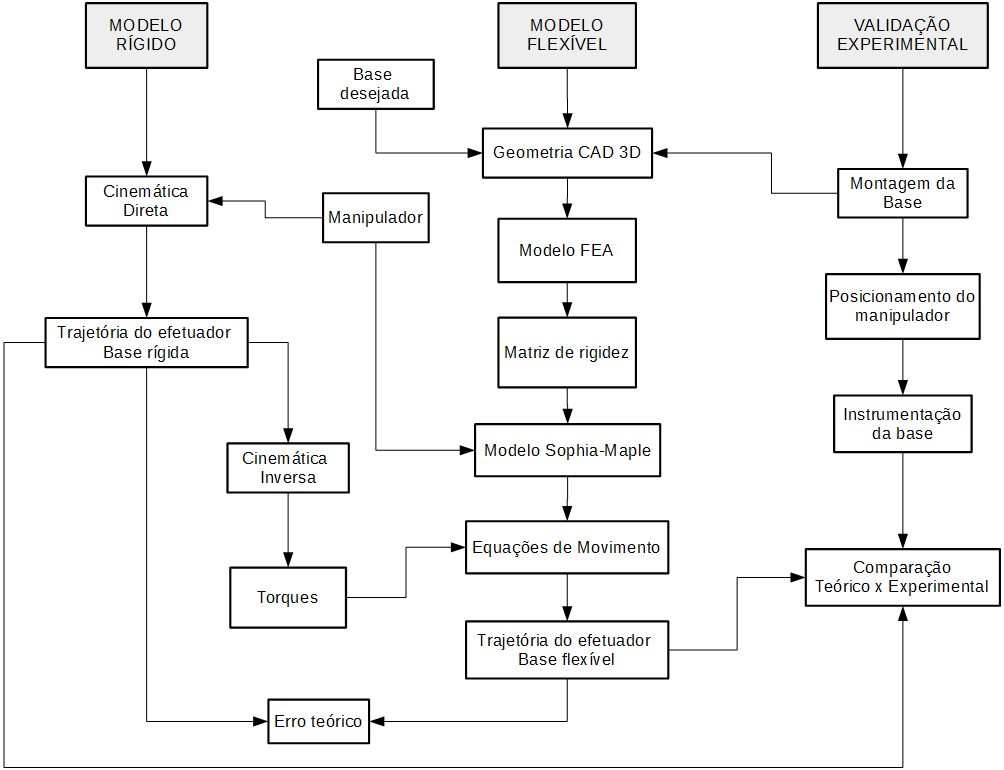
\includegraphics[width=15cm]{figs/diagrama.PNG}
\caption{Diagrama de etapas do método, Fonte: Autoria própria}
\label{fig::diagrama}
\end{figure}

\section{Fase 1: Pesquisa e viabilidade técnica}

Os primeiros 12 meses da primeira fase do projeto EMMA estudaram o Estado da
Arte para robôs de serviço, de pequeno a médio porte, utilizados em processos de
revestimento por HVOF.
A partir daí possibilitou-se o estudo da viabilidade técnica de se trasportar e
posicionar um robô dentro do espaço confinado de uma turbina, a fim de realizar
a manutenção do revestimento das pás. A figura~\ref{fig::turbina}
apresenta um desenho da turbina da Usina Hidrelétrica de Jirau-RO, onde o
protótipo EMMA será aplicado.

\begin{figure}[h!]
\centering
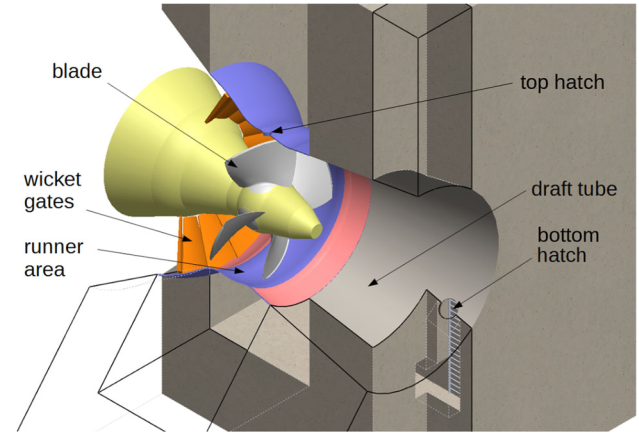
\includegraphics[width=10cm]{figs/turbina.PNG}
\caption{Turbina tipo Kaplan da UHE-Jirau, Fonte:~\citet{Freitas2017}}
\label{fig::turbina}
\end{figure}

Nesta etapa atestou-se a viabilidade da solução utilizando-se o acesso da
escotilha inferior para entrada do manipulador e dos equipamentos necessários
para montagem do sistema. 

Escolheu-se o modelo MOTOMAN MH12, da fabricante YASKAWA -- um manipulador
antropomórfico que contém 6 juntas de rotação em cadeia aberta -- por ser capaz
de entrar pelo acesso de escotilha e atender aos requisitos impostos pelo
processo de revestimento.

Definiu-se também a base sendo composta por seções modulares a serem montadas no interior da turbina para formar uma estrutura que  fornece 3 graus de liberdade para o posicionamento do robô em frente às
pás. Os módulos são compostos por perfis de alumínio estrutural e trilho,
formando uma junta prismática. Dois trilhos sobrepostos por meio de uma junta
rotacional, conferem os graus de liberdade necessários, numa configuração PRP
(Prismático-Rotacional-Prismático).
Braços de ancoragem com terminação em bases magnéticas ou copos de sucção são distribuídos a partir da
base para se obter maior rigidez da estrutura. 

A figura~\ref{fig::modulo} ilustra o o conceito da estrutura que forma a base e
destaca a composição de dois módulos que compõem a esturura.

\begin{figure}[h!]
\centering
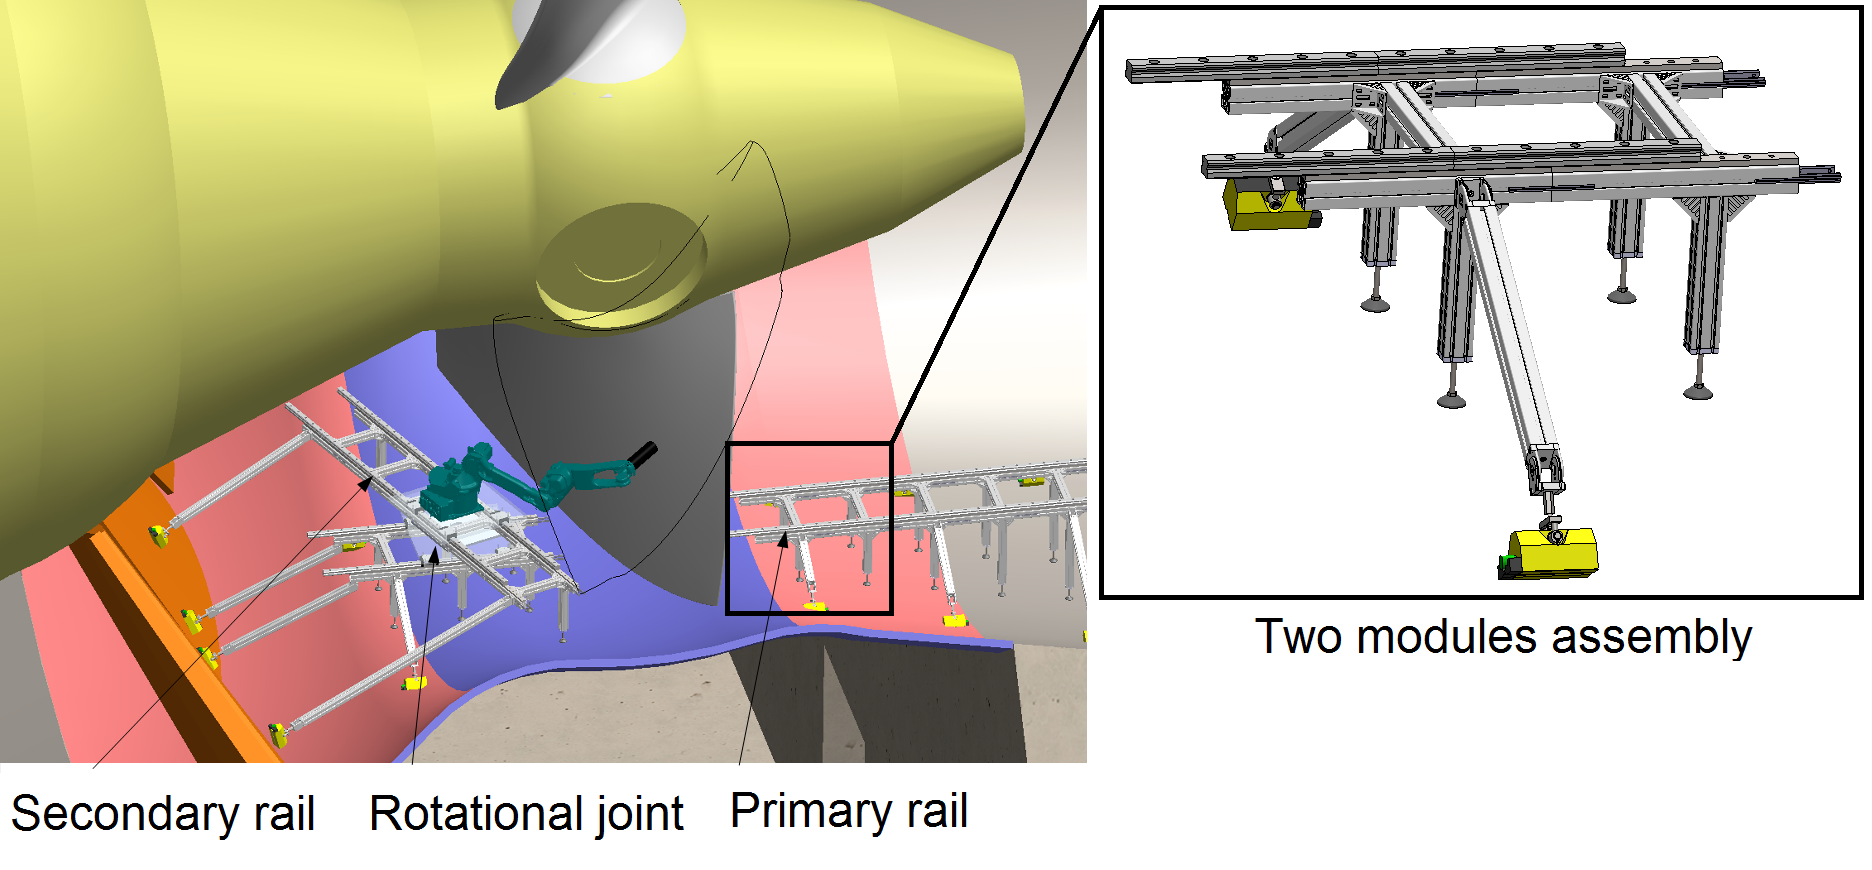
\includegraphics[width=12cm]{figs/modulo.PNG}
\caption{Base com o robô e módulo em detalhe, Fonte:~\citet{Freitas2017}}
\label{fig::modulo}
\end{figure}

\section{Fase 2: Detalhamento e simulações}

A segunda fase do projeto EMMA iniciou-se em Julho de 2016. Esta fase tem o
objetivo de detalhar a solução proposta, a fim de implementá-la ao final
do projeto, com um primeiro protótipo fabricado. Nesta etapa será incluído o
modelo de base flexível que auxiliará no dimensionamento da estrutura e dos braços de
ancoragem, considerando as cargas dinâmicas do manipulador. 

Nesta etapa destaca-se também o modelamento da geometria em CAD de diferentes
configurações de base, uma para cada posição do robô e as simulações por MEF
para obtenção da Matriz de Rigidez em função dessas posições. 

Simulações no modelo dinâmico do Sophia-Maple permitirão avaliar a influência de
diferentes configurações de base, por fornecem diferentes Matrizes de Rigidez.

Obtém-se portanto a trajetória pelo modelo flexível, o que permite verificar seu impacto no cumprimento dos requisitos de trajetória e velocidade
que o processo de revestimento HVOF requer.

\begin{figure}
\centering
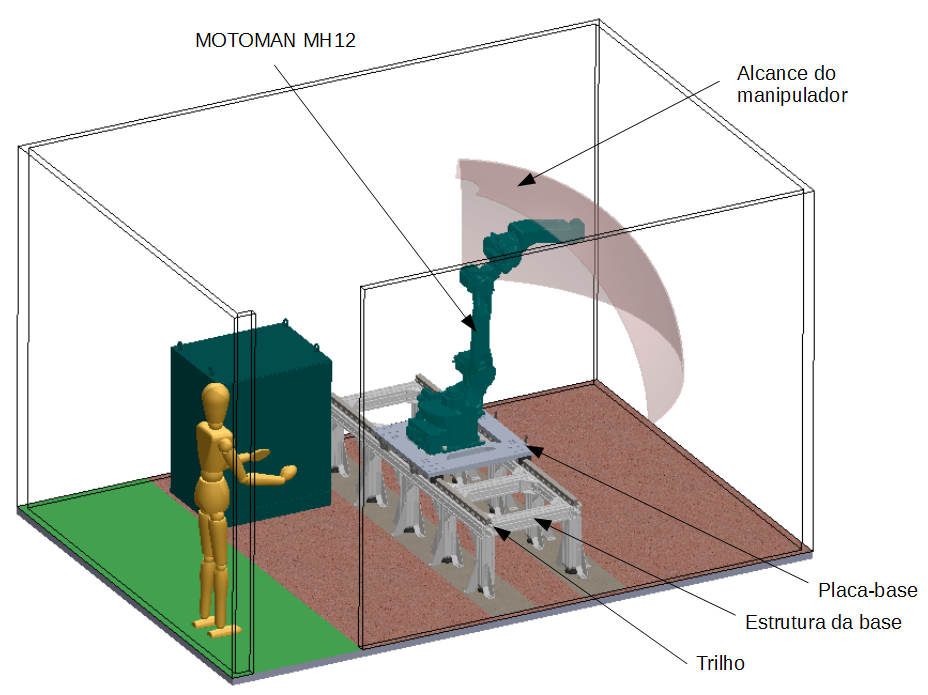
\includegraphics[width=10cm]{figs/sala_testes.PNG}
\caption{Sala de testes do manipulador, Fonte: Autoria própria}
\label{fig::base_teste}
\end{figure}

\section{Fase 3: Experimento e resultados}

O porjeto EMMA prevê uma etapa de testes de controle, trajetória, segurança,
software, interface de usuário e da base do robô. Para isso, foi montado um
laboratório de testes na empresa THIRTEEN ROBOTICS, para instalação do
manipulador em uma estrutura similar à projetada para a solução
\textit{in situ}.
Acelerômetros instalados na estrutura e alinhados com um sistema de referência
permitirão avaliar as acelerações em cada direção.
Uma trajetória idêntica a utilizada nas simulações dos modelos teóricos será
programada. Os dados de acelerações ao longo do tempo em que o robô realiza a
tarefa serão guardados e tratados para comparação com os outros
modelos.

\section{Fase 4: Discussão, redação e revisão}

A fase 4 compreende a etapa de discussão dos resultados obtidos, levando a
considerações sobre a efetividade do método proposto e trabalhos futuros.
Reserva-se esta etapa também para a revisão e redação da dissertação, e
formatação final do documento.




  \chapter{Cronograma}

A seguir é apresentado um cronograma compreendendo as 4 fases
do projeto e os principais marcos em cada fase. Os dois primeiros anos foram
separados em trimestres e, a partir de 2017, em semanas. Ao final de
cada etapa está prevista a redação de um tópico da dissertação final. Destaca-se
ainda os marcos com datas específicas, na última coluna.


\newpage


\begin{figure}
\centering
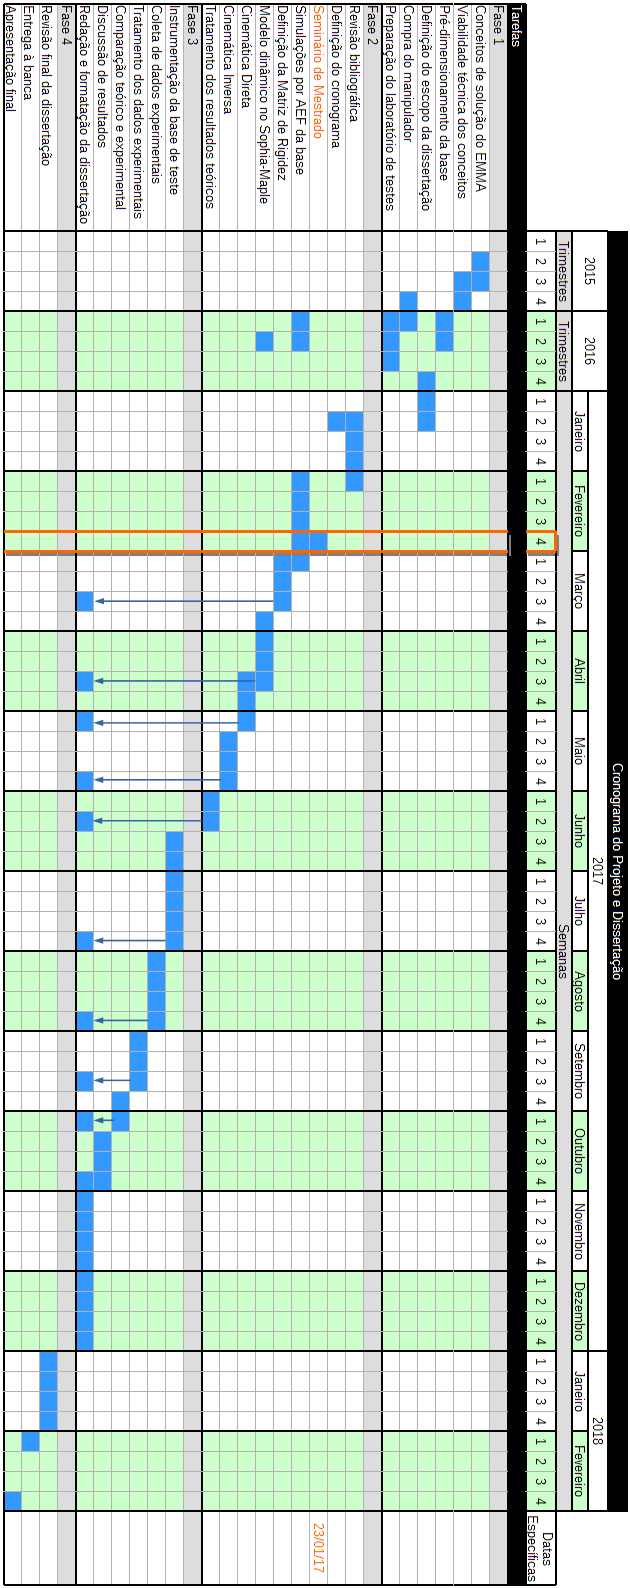
\includegraphics[width=10cm]{figs/cronograma.PNG}
%\caption{Cronograma}
\label{fig::cronograma}
\end{figure}


   \backmatter
   \bibliographystyle{coppe-unsrt}
   \renewcommand\bibname{Referências}
   \bibliography{thesis}

%   \appendix
%   \chapter{Algumas Demonstra{\c c}\~oes}

  \end{document}
